\iffalse
\documentclass[10pt,a4paper]{report}
\usepackage[utf8]{inputenc}
\usepackage{amsmath}
\usepackage{amsfonts}
\usepackage{amssymb}
\usepackage{graphicx}
\usepackage{multicol}
\usepackage{tabularx}
\usepackage{tikz}
\newcommand{\myvec}[1]{\ensuremath{\begin{pmatrix}#1\end{pmatrix}}}
\let\vec\mathbf
\let\myvec\bf
\providecommand{\mtx}[1]{\mathbf{#1}}
\newcommand{\mydet}[1]{\ensuremath{\begin{vmatrix}#1\end{vmatrix}}}
\usetikzlibrary{arrows,shapes,automata,petri,positioning,calc}
\usepackage{hyperref}
\usepackage{tikz}
\usetikzlibrary{matrix,calc}
\usepackage[margin=0.5in]{geometry}
\providecommand{\norm}[1]{\left\lVert#1\right\rVert}
\let\vec\mathbf
\newenvironment{Figure}
  {\par\medskip\noindent\minipage{\linewidth}}
  {\endminipage\par\medskip}
    
 
 
\begin{document}
%--------------------logo figure-------------------------%
\begin{figure*}[!tbp]
  \centering
  \begin{minipage}[b]{0.4\textwidth}
    \end{minipage}
  \hfill
  \vspace{5mm}\begin{minipage}[b]{0.4\textwidth}

  \end{minipage}\vspace{0.2cm}
\end{figure*}
%--------------------name & rollno-----------------------
\raggedright \textbf{Name}:\hspace{1mm} Varsha Reddy\hspace{3cm} \Large \textbf{Assignment-4}\hspace{2.5cm} % 
\normalsize \textbf{Roll No.} :\hspace{1mm} FWC22038\vspace{1cm}
\begin{multicols}{2}

\raggedright \textbf{PROBLEM:}\vspace{2mm}\\
\fi
In Fig.
		\ref{fig:9/9/4/3}
	\begin{figure}[!h]
		\centering
 \includegraphics[width=\columnwidth]{chapters/9/9/4/3/figs/ABC.pdf}
		\caption{}
		\label{fig:9/9/4/3}
  	\end{figure}
	$ABCD, DCFE$ and $ABFE$ are parallelograms. Show that   
	\begin{align}
	ar(ADE) = ar(BCF)
		\label{eq:9/9/4/3}
	\end{align}
	\begin{proof}
		From the given information and Appendix
	  \ref{eq:two-pgm},
  \begin{align}
		\label{eq:9/9/4/3/1}
	  \vec{B}-\vec{A} &= \vec{C} -\vec{D}
	  \\
		\label{eq:9/9/4/3/2}
	  \vec{C}-\vec{D} &= \vec{F} -\vec{E}
	  \\
		\label{eq:9/9/4/3/3}
	  \vec{B}-\vec{A} &= \vec{F} -\vec{E}
  \end{align}
  Thus, from  Appendix
  \ref{prop:pgm2d},
\begin{align}
	ar(ADE)  &= 
	\norm{\brak{\vec{D}-\vec{E}} \times \brak{\vec{D}-\vec{A}}}
	\\
	& = 
	\norm{\brak{\vec{C}-\vec{F}} \times \brak{\vec{C}-\vec{B}}}
	\\
	&=	ar(ADE) 
  \end{align}
  upon substituting from 
		\eqref{eq:9/9/4/3/1}
		and 
		\eqref{eq:9/9/4/3/2}.
	\end{proof}
	\iffalse
\vspace{0.5cm}\raggedright \\
Theory:
Parallelograms on the same base and in between the same parallels are equal in area.\\
Given: ABCD,DCFE and ABFE are parallelograms.
\vspace{2mm} \\ 
%----------------Solution  statement--------------%
\raggedright \textbf{Solution Statement:}\vspace{2mm}
\raggedright \\We can see that the sides of a triangle ADE and BCF are also the opposite sides of a given parallelogram. Now we can show both the triangles are congruent using congruency property. We know that congruent triangles are equal areas.  \\
\vspace{5mm}
\section{Construction}
  \begin{center}
   %\includegraphics[scale=1]{assignment4/ABC.pdf}
     \includegraphics[scale=0.5]{ABC.pdf} 
     Figure of Construction
   \end{center}
   \vspace{5mm}

\section{Table :}

The input parameters for this construction are 
\begin{center}
\begin{tabular}{|c|c|c|}
	\hline
	\textbf{Symbol}&\textbf{Value}&\textbf{Description}\\
	\hline
	a&3&EA\\
	\hline
	b&4.5&EF\\
	\hline
	c&2&ED\\
	\hline
	${\theta}_1$& 1$\pi/3$&$ \angle $AEF\\ 
	\hline
	${\theta}_2$& 2$\pi/3$&$ \angle $DEF\\ 
	    \hline
	E&$\
	\begin{pmatrix}
		0 \\
		0 \\
	\end{pmatrix}$%
	&Point E\\
	\hline
\end{tabular}
\end{center}

1. Considering point 'E' as origin.\\
2. From E,with some angle of 60 degrees,mark the point 'A'.\\
3. From E,with some angle of 120 degrees,mark the point 'D'.\\
4. With the distance of 'b' locate the point 'F'.\\
5. To locate a point 'B'\\
\begin{center}
    \myvec{ B = A+F-E }
\end{center}
6. To locate a point 'C'\\
\begin{center}
    \myvec{ C = D+F-E }
\end{center}
7. Joining all the lines from the figure.
\vspace{0.5cm}\\
%-----------------------------solution---------------------------
 \section{Solution}
% \vspace{2mm}\\
n ABCD,
\begin{equation}
\vec{A-B}=\vec{D-C}
\end{equation}
\begin{equation}
\vec{A-D}=\vec{B-C}
\end{equation}
\\
In DEFC,
\begin{equation}
\vec{D-C}=\vec{E-F}
\end{equation}
\begin{equation}
\vec{D-E}=\vec{C-F}
\end{equation}
\\
In ABEF,
\begin{equation}
\vec{A-B}=\vec{E-F}
\end{equation}
\begin{equation}
\vec{A-E}=\vec{B-F}
\end{equation}

\vspace{1mm}

\textbf{To Prove:} 
  \begin{center}
  \begin{equation}
      \vec{Ar(ADE)=Ar(BCF)}
  \end{equation}
 \vspace{3mm}
 Area of the triangle $\Delta$ADE is given by \\
 Ar($\Delta$ADE) 
\begin{equation} 
 = \frac{1}{2}\norm{\vec{A-D}\times\vec{D-E}}
\end{equation}
  %\vspace{3mm}
 \vspace{3mm}
  Area of the triangle $\Delta$BCF is given by \\
  Ar($\Delta$BCF)
   \begin{equation}
   =\frac{1}{2}\norm{\vec{B-C}\times\vec{C-F}}
   \end{equation}
 \end{center}
 substituiting (2) and (4) in (9),
 \begin{equation}
   =\frac{1}{2}\norm{\vec{A-D}\times\vec{D-E}}
   \end{equation}
   from (8) and (10),
 \begin{center}
\begin{equation}
    \vec{Ar(ADE)=Ar(BCF)}
\end{equation}
\end{center}
The below python code realizes the above construction: \\
\url{https://github.com/9705701645/FWC/blob/main/lines4.py}
\bibliographystyle{ieeetr}
\end{multicols}
\end{document}
\fi
